\documentclass{article}
\usepackage{pgfplots}
\usepackage{hyperref}
\usepackage{amsmath}
\usepackage{amsfonts}
\usepackage{amssymb}
\usepackage{graphicx}
\usepackage{listings}
\usepackage{float}
\usepackage{tikz}
\usepackage{circuitikz}
\usepackage{color}
\renewcommand{\labelenumi}{\arabic{enumi}.}
\renewcommand{\labelenumii}{\arabic{enumi}.\arabic{enumii}}
\usepackage{enumitem}
\definecolor{mauve}{RGB}{204,153,255}
\definecolor{mylilas}{RGB}{200,162,200}
\definecolor{pageno}{gray}{0.30}

\title{Physics Problem Set 3} \date{22-09-2015} \author{Hrishi Olickel}

\begin{document}
 \pagenumbering{gobble}
 \maketitle
 \pagenumbering{arabic}
 \newpage
 
 \graphicspath{ {/} }
\lstdefinestyle{MATLAB}{ % 
    %basicstyle=\color{red},
    language = Matlab,
    breaklines=true,%
    morekeywords={matlab2tikz},
    frame=single,
    keywordstyle=\color{blue},%
    morekeywords=[2]{1}, keywordstyle=[2]{\color{black}},
    identifierstyle=\color{black},%
    stringstyle=\color{mylilas},
    commentstyle=\color{green},%
    showstringspaces=false,%without this there will be a symbol in the places where there is a space
    numbers=left,%
    numberstyle={\tiny \color{black}},% size of the numbers
    numbersep=9pt, % this defines how far the numbers are from the text
    emph=[1]{for,end,break},emphstyle=[1]\color{red}, %some words to emphasise
    %emph=[2]{word1,word2}, emphstyle=[2]{style},    
} 

\lstset{style=MATLAB}

\section{Answers}

\begin{enumerate}
	\item Done reading.
	\item Done reading.

	\item	
		We know that $V = Q/C$,
		and n this case when the switch is thrown to the left,
		\begin{equation} V_1 = 16.0 V \end{equation}
		\[C_1 = 4.00 \mu F\]
		\[Q_1 = V_1 \times C_1 = 64.0 \mu C \]
		When the switch is thrown to the right, this charge $Q_1$ is redistributed among the capacitors. We know the following about this system:
		\begin{equation} V_{23} = V_1 \end{equation}
		\begin{equation} Q_1 = Q_{1new} + Q_{23} \end{equation}
		We then find the combined capacitance of $C_2$ and $C_3$: 
		\[ C_{2+3} = (\frac{1}{C_2}+\frac{1}{C_3})^{-1} = 2.0 \mu F \]
		From (2), we can now find the ratio of the new charge distribution:
		\[ \frac{Q_{1new}}{C_1} = \frac{Q_{23}}{C_{2+3}} \]
		\[ \therefore Q_{1new} = 2 \times Q_{23} \]
		From this, we can now find that
		\begin{enumerate}[label=(\alph*)]
			\item The final charge on capacitor 1:
				\[ Q_{1new} = \frac{2}{3} \times Q_1 \]
				\[ Q_{1new} =  42.6 \mu C \]
			\item Final charge on capacitor 2:
				\[ Q_{2} = \frac{1}{3} \times Q_1 \]
				\[ Q_{2} =  21.3 \mu C \]
			\item Since capacitor 2 and 3 are in parallel, we know that the magnitude of the charge across both of them must be the same. Hence:
				\[ Q_{3} = 21.3 \mu C \] 
		\end{enumerate}
		
	\item
		\begin{enumerate}[label=(\alph*)]
		\item The easiest way to build the resistance network when you know the desired value is to start with a decade-counter setup, whereby you have multiple units of resistance of values $1 \Omega$, $0.1 \Omega$ and $0.01 \Omega$. We can achieve this by having 1, 10 and 100 resistances of value $1 \Omega$ in parallel, respectively. Once this is done, we can simply combine them in the number we need such that the total resistance equals $1.41 k\Omega$. However, in this case, it would require a large number of resistors. We could simply use a resistance ladder in order to make this work, and an extension of this ladder, as we will see in (b), can solve for the square root of 2 to infinity.
		We have the following network:
		\begin{figure}[h!]
  			\begin{center}
    				\begin{circuitikz}
      					\draw (0,0) node[anchor=east] {$b$}
      					to[R=R] (2,0) % The resistor
      					to[short] (4,0) node[anchor=north] {$d$}
					to[short] (4,1)
					to[short] (3,1)
					to[R=R] (3,3)
					to[short] (4,3)
					to[short] (4,4) node[anchor=south] {$c$}
					to[short] (0,4) node[anchor=east] {$a$};
					\draw (4,1)
					to[short] (5,1)
					to[R=R] (5,3)
					to[short] (4,3);
					\draw (4,0)
					to[R=R] (7,0)
					to[short] (7,1) node[anchor=south] {$e$}
					to[short] (6,1)
					to[R=R] (6,3)
					to[short] (7,3) node[anchor=north] {$f$}
					to[short] (7,4)
					to[R=R] (4,4);
					\draw (7,1)
					to[short] (8,1)
					to[R=R] (8,3)
					to[short] (7,3);
    				\end{circuitikz}
    				\caption{Basic Unit}
  			\end{center}
		\end{figure}
		
		When $R = 1 k\Omega$, 
		\[ R_{fe} = \frac{1}{R} = 500 \Omega \]
		\[ R_{cd} = \frac{2.5 k\Omega \times 0.5 k\Omega}{2.5 k\Omega + 0.5 k\Omega}  = 0.41\overline{6} k\Omega \]
		\[ R_{ab} = 1 k\Omega + R_{cd} \approx 1.41 k\Omega \] 
		
		\item We can simply extend this ladder to find the resistance of $\sqrt{2}$ to any precision we require, as follows:
		\begin{figure}[H]
  			\begin{center}
    				\begin{circuitikz}
      					\draw (0,0) node[anchor=north] {$f$}
      					to[R=$R_1$] (2,0)
      					to[short] (4,0)
					to[short] (4,1)
					to[short] (3,1)
					to[R=R] (3,3)
					to[short] (4,3)
					to[short] (4,4) 
					to[short] (0,4) node[anchor=south] {$e$};
					\draw (4,1)
					to[short] (5,1)
					to[R=R] (5,3)
					to[short] (4,3);
					\draw (4,0)
					to[R=R] (7,0) node[anchor=north] {$d$}
					to[short] (7,1) 
					to[short] (6,1)
					to[R=R] (6,3)
					to[short] (7,3) 
					to[short] (7,4) node[anchor=south] {$c$}
					to[R=R] (4,4);
					\draw (7,1)
					to[short] (8,1)
					to[R=R] (8,3)
					to[short] (7,3);
					\draw (7,0)
					to[R=R] (10,0)
					to[short] (10,1)
					to[short] (9,1)
					to[R=R] (9,3)
					to[short] (10,3)
					to[short] (10,4)
					to[R=R] (7,4);
					\draw (10,1)
					to[short] (11,1)
					to[R=R] (11,3)
					to[short] (10,3);
					\draw (10,0) node[anchor=north] {$b$}
					to[short] (12,0);
					\draw (10,4) node[anchor=south] {$a$}
					to[short] (12,4);
    				\end{circuitikz}
    				\caption{Basic Unit}
  			\end{center}
		\end{figure}		
		If we repeate the segment of the circuit between $a-b$, we can adjust the precision to which the $\sqrt{2}$ can be found. Let's prove this:
		Assuming this ladder to extend to infinity, we can then make this reasonable assumption -
	 	\begin{equation} R_{cd} = R_{ef} \end{equation}
		Forgetting the initial resistor $R_1$, we get the following:
		\[ R_{ef} = 2 + 0.5 || R_{cd} \]
		From (4), 
		\[ R_{ef} = 2 + 0.5 || R_{ef} \]
		Simplifying, we get
		\[ R_{ef}^2 - 2 R_{ef} - 1 = 0 \]
		Solving,
		\[ R_{ef} = \sqrt{2} - 1 \]
		Adding $R_1$, we get
		\[ R_{total} = \sqrt{2} \]
		\end{enumerate}
		\item 
		\begin{enumerate}[label=(\alph*)]
		\item 
		If we consider effective voltage and capacitance as across $R_3$:
		\[ R_{eff} = (R_{1}+R_{2}) || R_3 \]
		\[ R_{eff} = 7.5 k \Omega \]
		
		\item
		\[ C_{eff} = 5.0 \mu F || 10.0 \mu F \]
		\[ C_{eff} = \frac{10.0 \times 5.0}{10.0 + 5.0} = 3.\overline{3} \mu F \]
		
		\item From the RC time constant we know that it takes approximately $0.7 RC$ to charge the capacitor to half capacity.
		If we ignore the current from the charging of one capacitor as affecting the charge time of the other, we find the following:
		\[ \tau = R_1 \times C_2 = R_2 \times C_1 = 5.0 \times 10^3 \Omega \times 10.0 \times 10^{-6} F \]
		\[ \tau =  0.05 s \]
		\[ 0.7 \tau = 0.035 s \]
		Upon simulating the circuit, we find that this holds true:
		\begin{figure}[H]
			\caption{Circuit Simulation}
			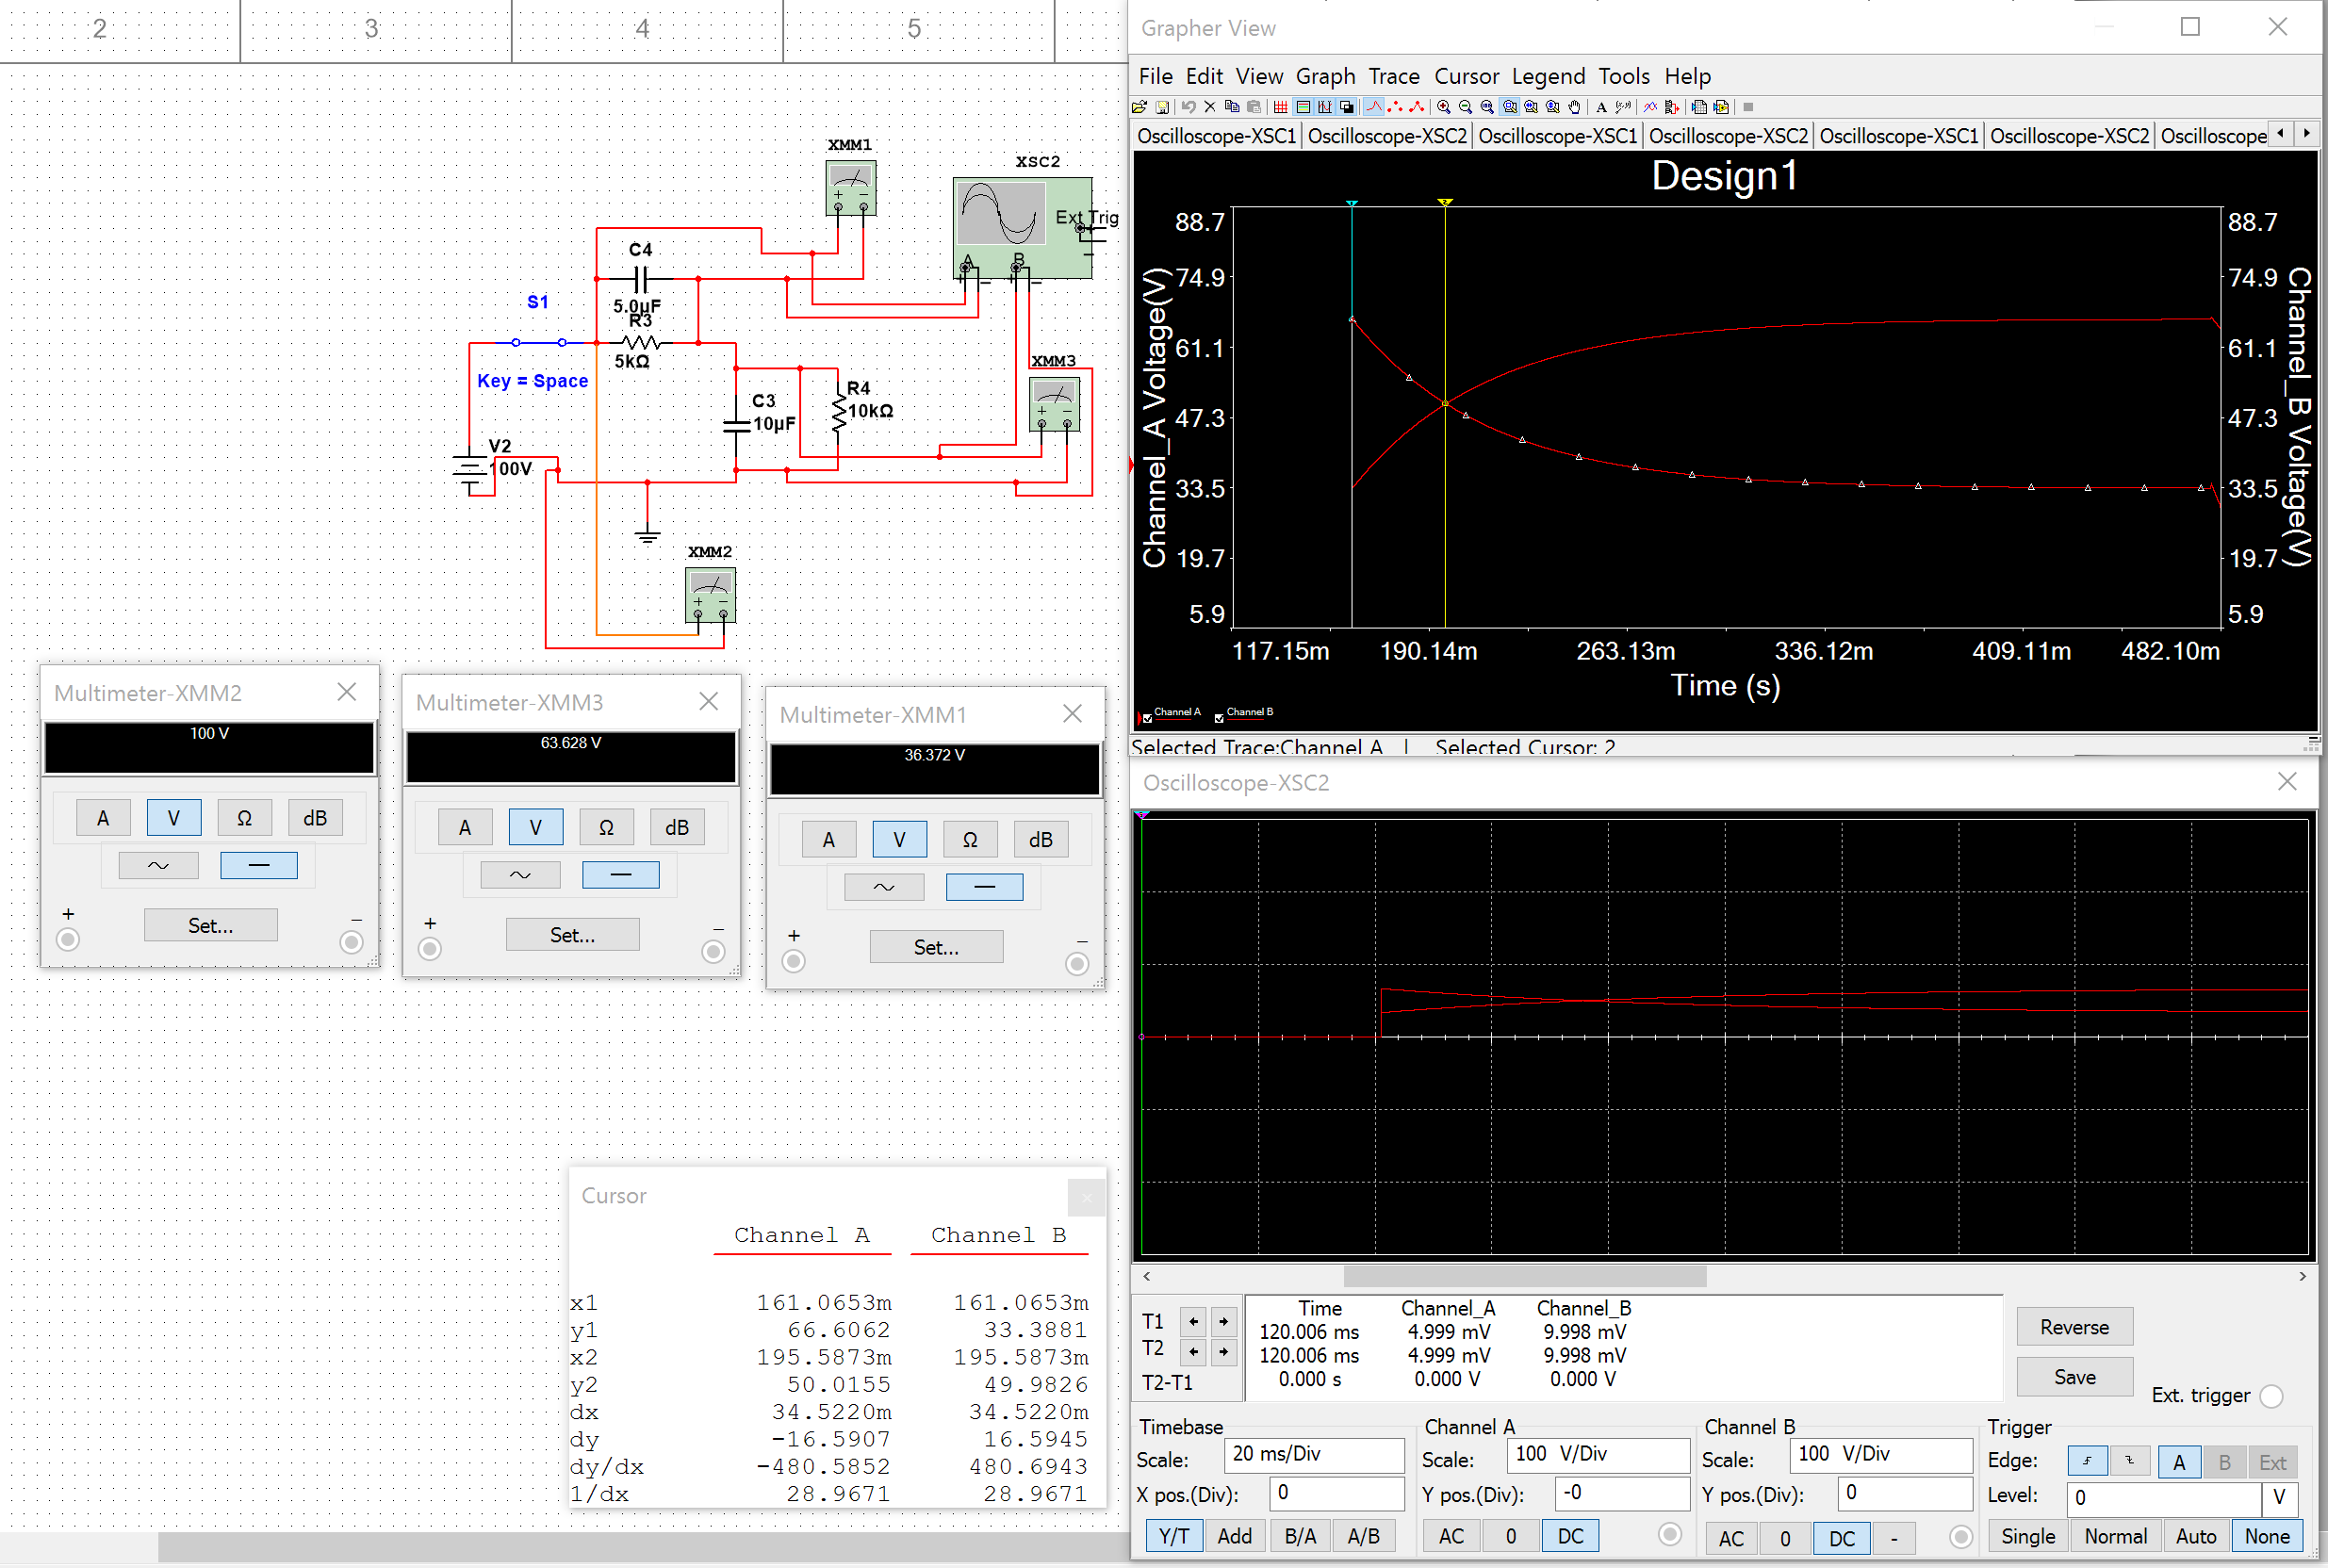
\includegraphics[width=\textwidth]{Simulation1}
		\end{figure}
		\begin{figure}[H]
			\caption{The Circuit}
			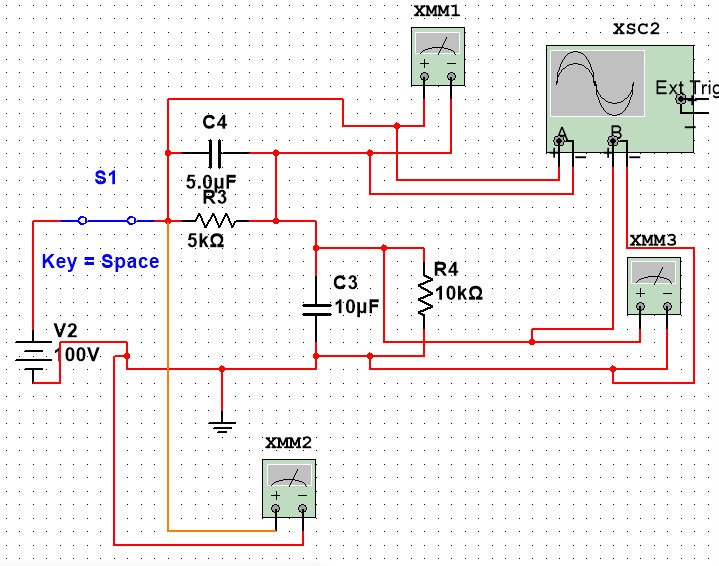
\includegraphics[width=\textwidth]{circuit}
		\end{figure}		
		\begin{figure}[H]
			\caption{Oscilloscope Reading}
			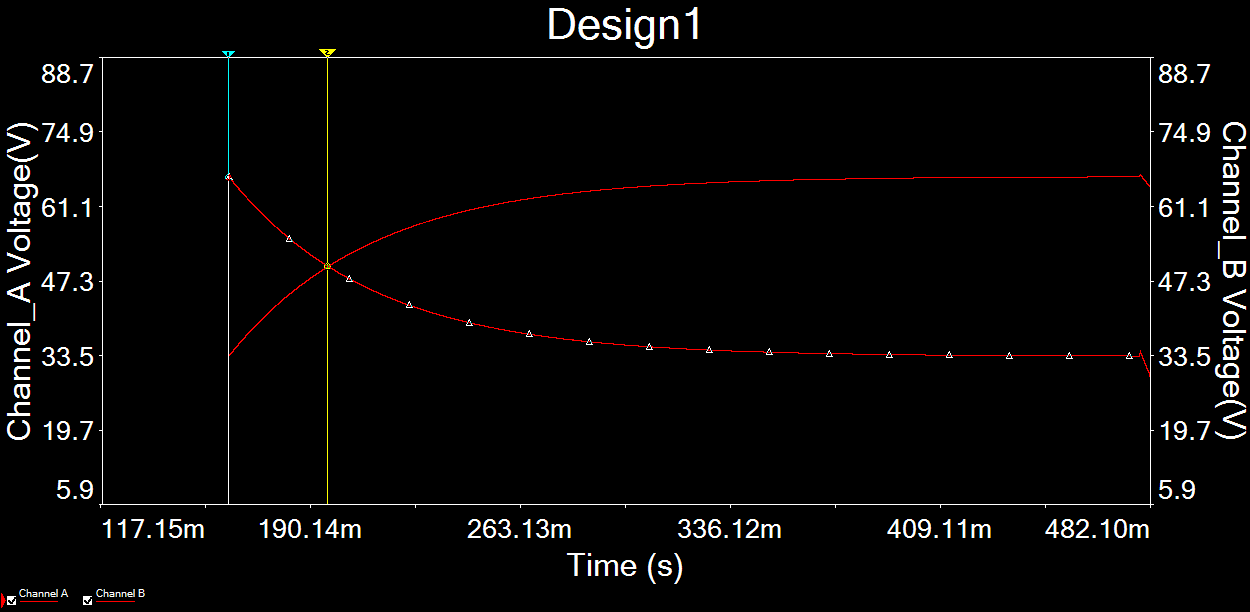
\includegraphics[width=\textwidth]{oscilloscope}
		\end{figure}
		\begin{figure}[H]
			\caption{Final Readings}
			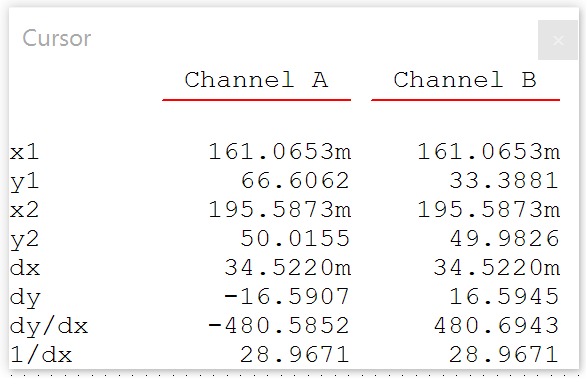
\includegraphics[width=\textwidth]{Cursor}
		\end{figure}
		\item When discharging, we need to consider $R_3$ as well:
		\[ \tau_{C2} = (R_1 + R_3) || R_2 \times C_2 = 6.66 k\Omega \times 10.0 \mu F \]
		\[ \tau_{C2} = 0.06 s \]
		\[ 0.7 \tau_{C2} = 0.04 s \]
		\[ \tau_{C1} = (R_2 + R_3) || R_1 \times C_2 = 6.66 k\Omega \times 10.0 \mu F \]
		\[ \tau_{C1} = 0.02 s \]
		\[ 0.7 \tau_{C2} = 0.015 s \]
		Likewise, simulation holds up the results.
		\end{enumerate}
		\item
		Let us consider the equation:
		\[ \dot{N} = rN(1-\frac{N}{K}) \]
		Very quickly, we can simulate this first-order ODE for a few starting values:
		\begin{figure}[H]
			\caption{Graph of N against T, K = 1000}
			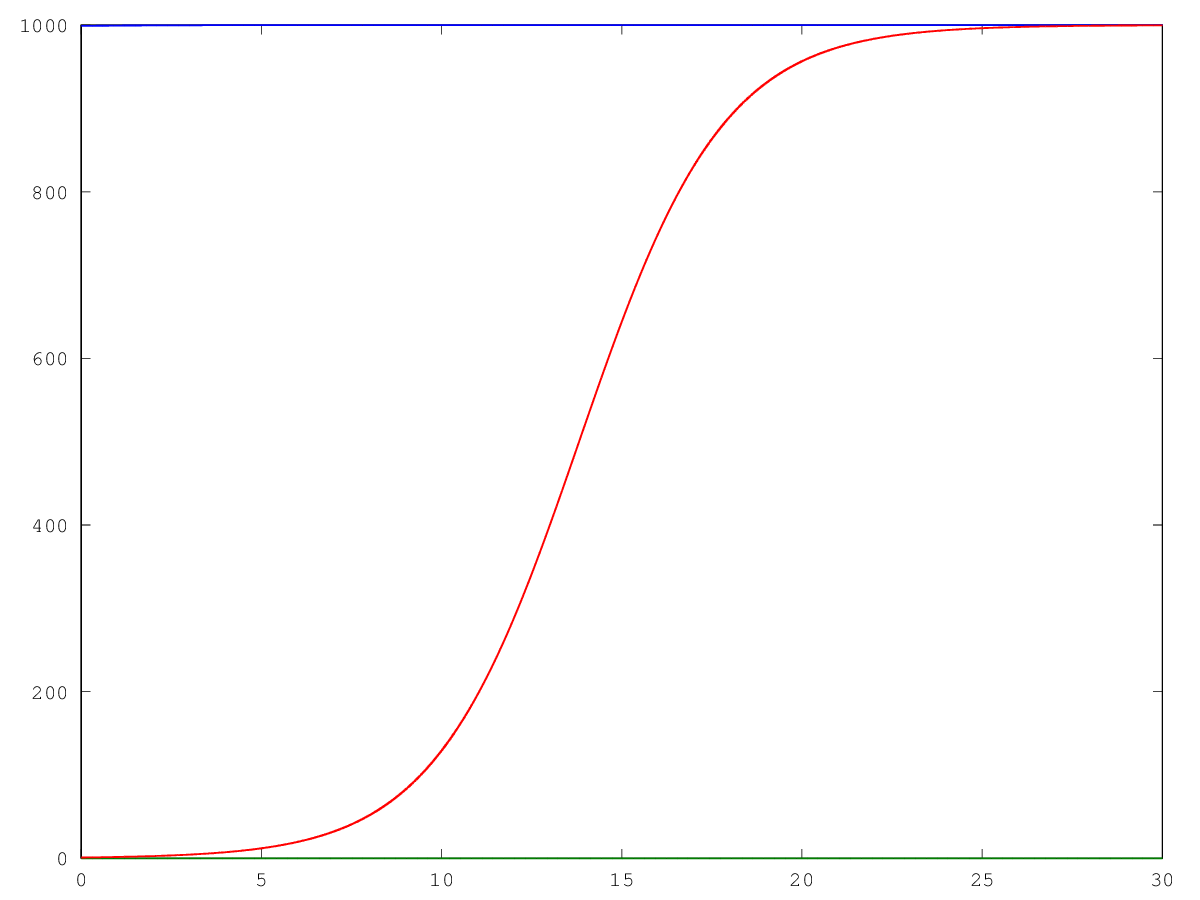
\includegraphics[width=\textwidth]{growthFunction}
		\end{figure}
		
		The simulation holds up the conclusions found in Strogatz. N=K is a stable fixed point, where disturbances in either direction will precipitate a return back to it. N=0 is the secondary fixed point, but it is unstable. A negative start value will upset the system whereby it will keep increasing with no fixed point, however when simulating a real populating system N<0 is impossible. Next we look at the flow on a line plot:
		\begin{figure}[H]
			\caption{Flow on a Line, $x_0=1$, K=1000 }
			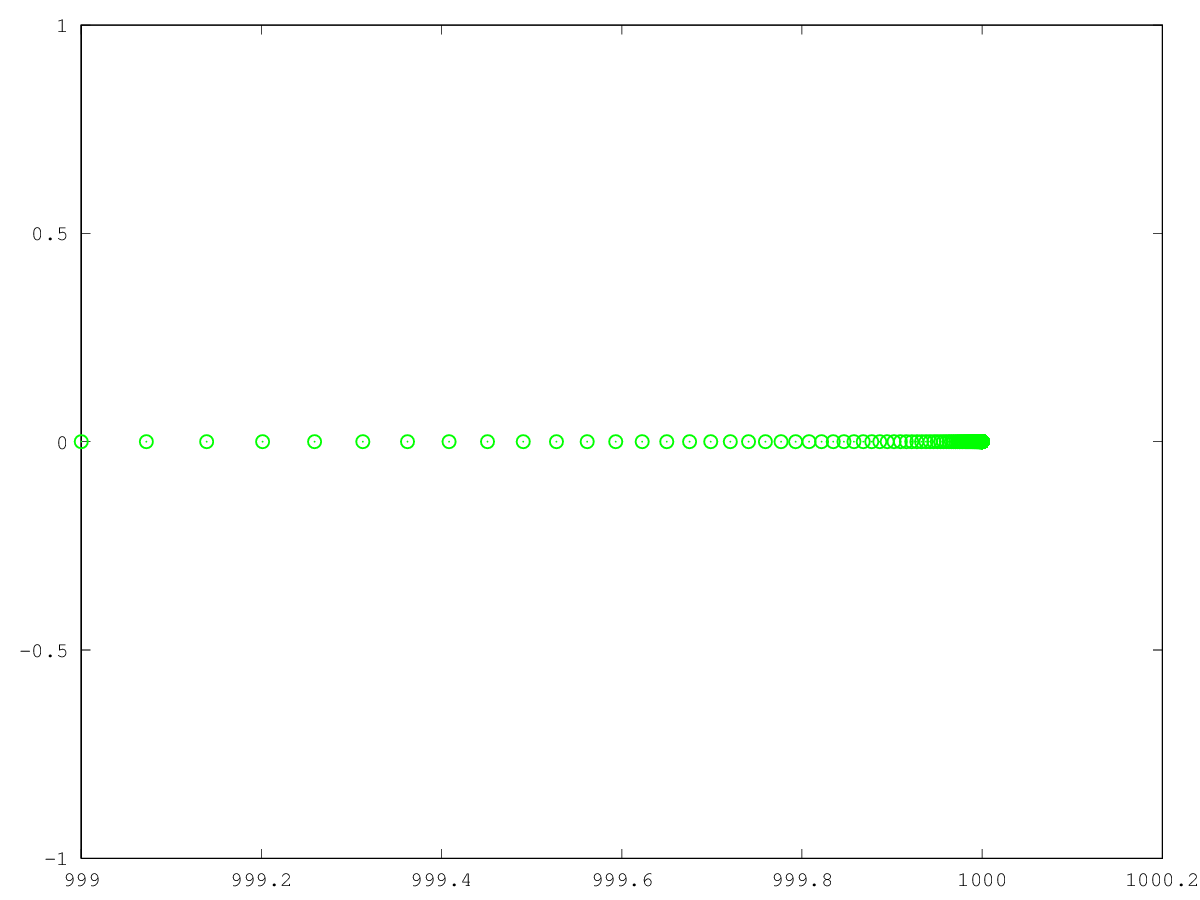
\includegraphics[width=\textwidth]{growthFunction3}
		\end{figure}
		
		Combining the different start values, we see the same result:
		\begin{figure}[H]
			\caption{Flow on a Line, $x_0=0,1,1000$, K=1000 }
			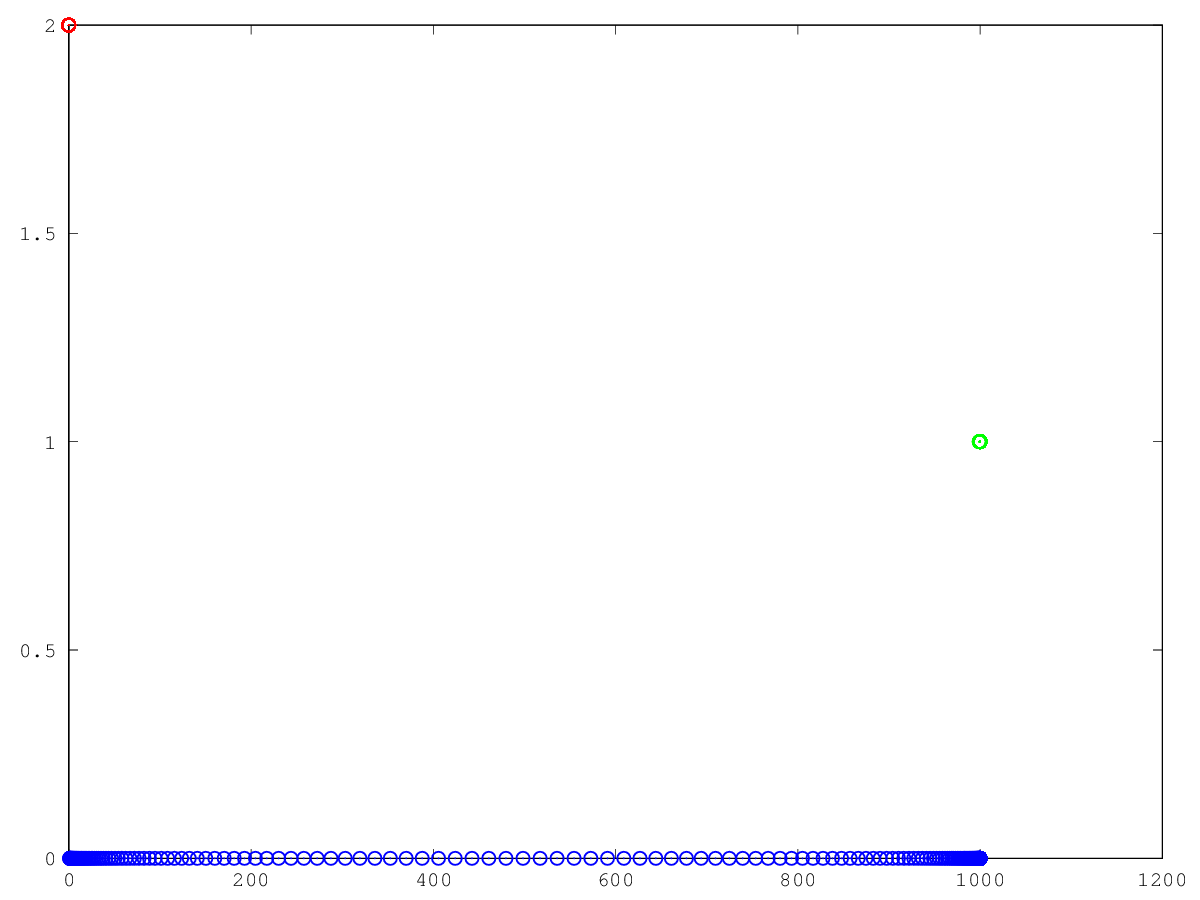
\includegraphics[width=\textwidth]{growthFunction2}
		\end{figure}
		
		From the analysis we can see how a stable fixed point can be added by the addition of the $(1-\frac{N}{K})$ term. However, it must be noted that even though N=0 is an unstable fixed point in the simulation of the system, it is not so when a real population is considered. A population of zero is has no chance of being altered, if the system is closed.
\end{enumerate}
\end{document}